\documentclass{ctexart}
\usepackage{ctex}
\usepackage{graphicx}

\graphicspath{{figures/}}

\title{计算机科学基础}
\author{Mr Wu}
\date{2019 年 4 月}

\begin{document}
	\maketitle
	\section{计算机早期历史}
	最早的计算设备是算盘。
	
	Computer最早指代职业,一群专门做计算的人,后来逐渐发展成指代机器。
	
	第一个可以做加减乘除的机器是步进计算器。
	
	二战时为了精准发射炮弹,需要计算弹道。此时通过查表来实现,但这样做局限性较大。于是Charles Barbage提出了差分机。在构造差分机期间,分析机的概念出现了,这是通用计算机的雏形。
	
	Lovelace给分析机写了假想程序,成为了第一位程序员。
	
	20世纪人口暴增,美国计划10年进行一次人口普查。若仅靠人工算力,需要13年才能完成一次人口普查。于是打孔卡片制表机被发明,仅用2.5年就完成了一次人口普查。此时企业意识到计算机的价值,可以提升劳动力,提高处理数据密集型任务的效率,从而提升利润。于是有人成立了一家制表机器公司,这家公司后来与其它公司合并,便有了日后大名鼎鼎的IBM。
	\section{电子计算机}
	随着社会的发展,要求更强的计算能力,柜子大小的计算机发展到房间大小。维护费用高,且易出错。
	
	继电器可以控制电路开关,但继电器有质量,无法快速开关。而且每秒只能翻转50次,难以解决复杂问题。继电器的另一个缺点是它会随着时间磨损。因此对于含有很多继电器的大型设备,故障率大大提高。同时机器会吸引虫子,这正是$ DEBUG $的由来。
	\section{布尔逻辑和逻辑门}
	使用二进制的原因:状态简单;已有数学基础。
	
	基本操作:与,或,非。高级操作:异或。
	
	异或操作的实现如图所示:
	
	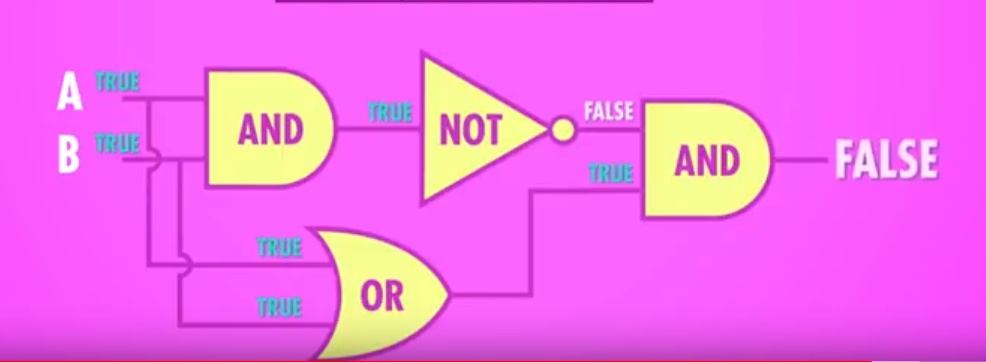
\includegraphics[scale=0.5]{NOR}
	\section{二进制}
	\section{算术逻辑单元}
	ALU包含一个算术单元和一个逻辑单元。算术单元用逻辑门处理加法。
	\section{寄存器}
	一组锁存器组成一个寄存器,一个寄存器能存储一个数字。
	
	64位寄存器需要64根数据线,64根连到输出端,加上一根允许写入线,共129根。
	
	解决方法是矩阵:对于256位的存储,只需要35根线。一根数据线,一根允许写入,一根允许读取,以及16行16列的线用于选取锁存器。
	
	256位内存的组成如图所示:
	
	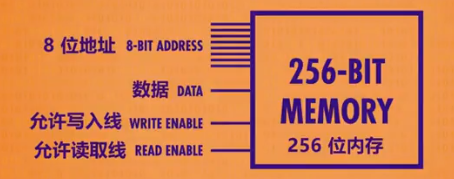
\includegraphics[scale=1]{Memory}
	
	\section{CPU}
	主板构造如图所示:
	
	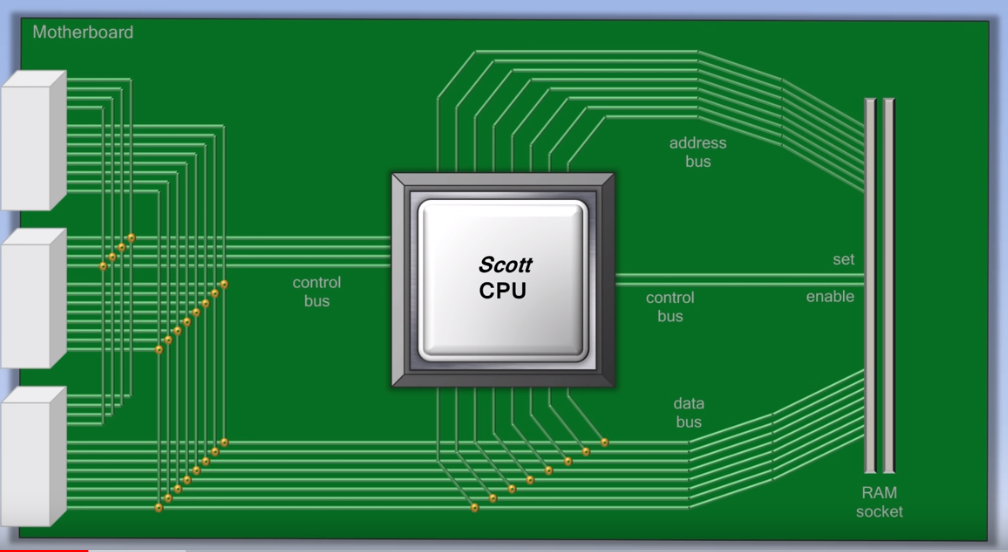
\includegraphics[scale=0.5]{CPU}
	
	计算机中主板负责连接所有组件。RAM是一个地址列表,每一个地址是一块数据,计算机通常从RAM中顺序提取并处理一块数据。
	
	当enable开启时,RAM向CPU发送一块数据,然后CPU处理这块数据。如果CPU想存数据,就要开启set。
	
	RAM中最重要的数据是指令,也包括数字,地址,字母等。每个CPU有一个指令集,CPU能够理解其中的指令。
	
	控制单元从RAM中接收指令,并将指令解析为具体的命令,让其它组件执行。其中最重要的组件是ALU,算术逻辑单元。
	
	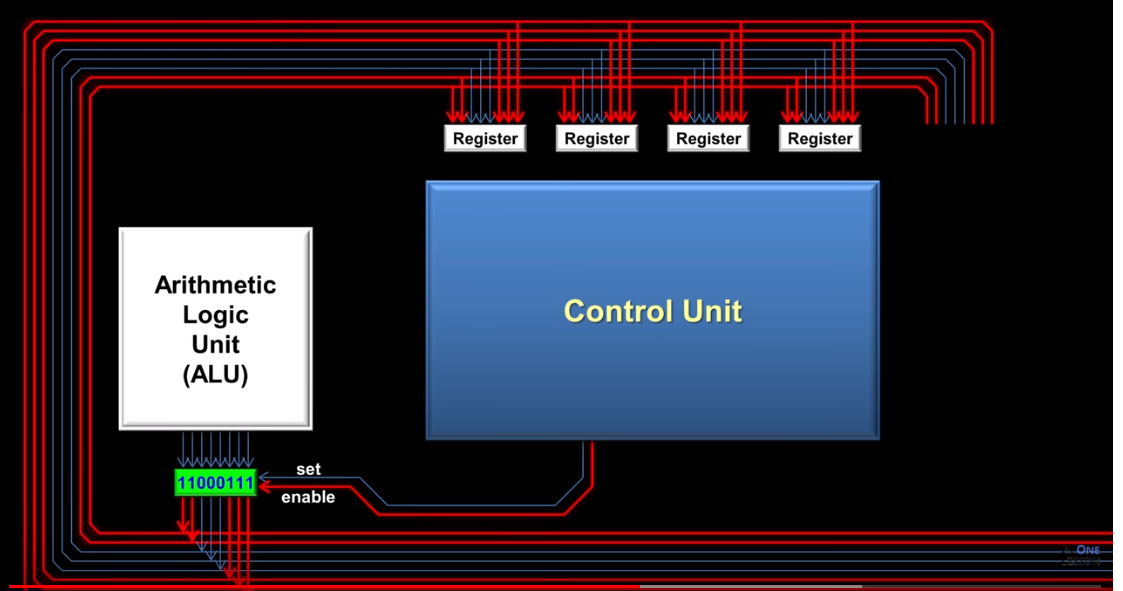
\includegraphics[scale=0.5]{CPU1}
	
	寄存器就像RAM一样,只不过它们在CPU内部,作用是临时存储数字。ALU将计算结果输出到寄存器,只有控制单元开启set时,寄存器才会保存结果。当控制单元开启enable时,寄存器将存储的结果输出到CPU总线。刚刚保存的结果沿着总线,发送到另一个寄存器中,这个寄存器可能已经存储了之前的计算结果。
	
	指令寄存器将指令传送到控制单元,然后控制单元告诉ALU该执行什么样的操作。执行完一条指令之后,需要将指令地址寄存器的set开启。
	
	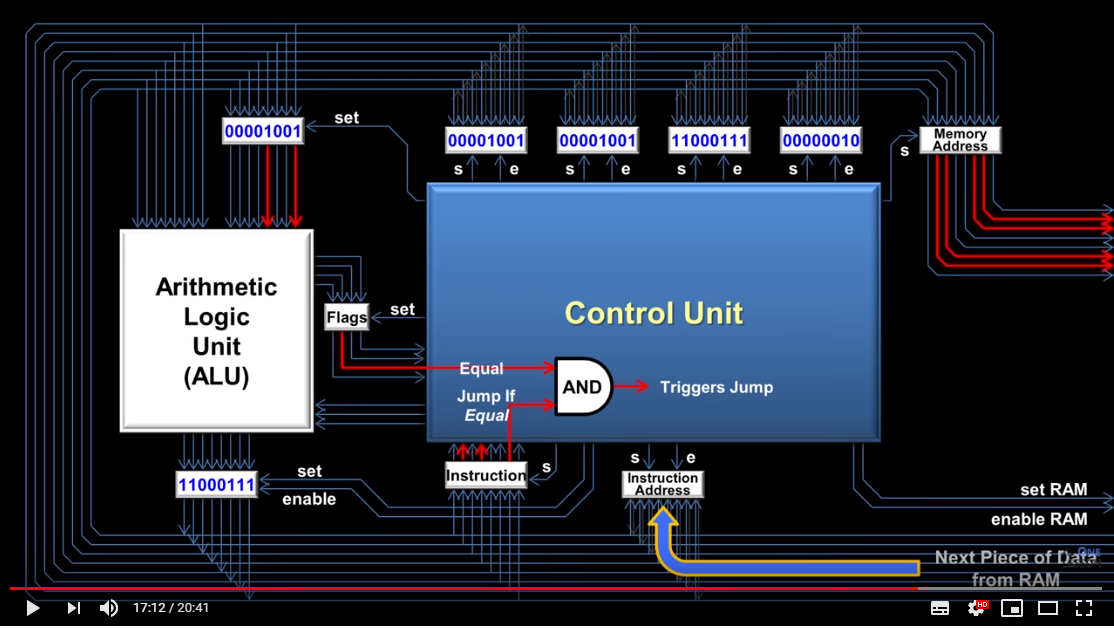
\includegraphics[scale=0.5]{CPU2}
\end{document}